\documentclass[12pt,letterpaper]{article}
\usepackage{graphicx,textcomp}
\usepackage{natbib}
\usepackage{setspace}
\usepackage{fullpage}
\usepackage{color}
\usepackage[reqno]{amsmath}
\usepackage{amsthm}
\usepackage{fancyvrb}
\usepackage{amssymb,enumerate}
\usepackage[all]{xy}
\usepackage{endnotes}
\usepackage{lscape}
\newtheorem{com}{Comment}
\usepackage{float}
\usepackage{hyperref}
\newtheorem{lem} {Lemma}
\newtheorem{prop}{Proposition}
\newtheorem{thm}{Theorem}
\newtheorem{defn}{Definition}
\newtheorem{cor}{Corollary}
\newtheorem{obs}{Observation}
\usepackage[compact]{titlesec}
\usepackage{dcolumn}
\usepackage{tikz}
\usetikzlibrary{arrows}
\usepackage{multirow}
\usepackage{xcolor}
\newcolumntype{.}{D{.}{.}{-1}}
\newcolumntype{d}[1]{D{.}{.}{#1}}
\definecolor{light-gray}{gray}{0.65}
\usepackage{url}
\usepackage{listings}
\usepackage{color}

\definecolor{codegreen}{rgb}{0,0.6,0}
\definecolor{codegray}{rgb}{0.5,0.5,0.5}
\definecolor{codepurple}{rgb}{0.58,0,0.82}
\definecolor{backcolour}{rgb}{0.95,0.95,0.92}

\lstdefinestyle{mystyle}{
	backgroundcolor=\color{backcolour},   
	commentstyle=\color{codegreen},
	keywordstyle=\color{magenta},
	numberstyle=\tiny\color{codegray},
	stringstyle=\color{codepurple},
	basicstyle=\footnotesize,
	breakatwhitespace=false,         
	breaklines=true,                 
	captionpos=b,                    
	keepspaces=true,                 
	numbers=left,                    
	numbersep=5pt,                  
	showspaces=false,                
	showstringspaces=false,
	showtabs=false,                  
	tabsize=2
}
\lstset{language=R}
\newcommand{\Sref}[1]{Section~\ref{#1}}
\newtheorem{hyp}{Hypothesis}

\title{Problem Set 4}
\date{Due: April 16, 2023}
\author{Applied Stats II}


\begin{document}
	\maketitle
	\section*{Instructions}
	\begin{itemize}
	\item Please show your work! You may lose points by simply writing in the answer. If the problem requires you to execute commands in \texttt{R}, please include the code you used to get your answers. Please also include the \texttt{.R} file that contains your code. If you are not sure if work needs to be shown for a particular problem, please ask.
	\item Your homework should be submitted electronically on GitHub in \texttt{.pdf} form.
	\item This problem set is due before 23:59 on Sunday April 16, 2023. No late assignments will be accepted.

	\end{itemize}

	\vspace{.25cm}
\section*{Question 1}
\vspace{.25cm}
\noindent We're interested in modeling the historical causes of infant mortality. We have data from 5641 first-born in seven Swedish parishes 1820-1895. Using the "infants" dataset in the \texttt{eha} library, fit a Cox Proportional Hazard model using mother's age and infant's gender as covariates. Present and interpret the output.



\begin{lstlisting}[language=R]
install.packages("eha")
install.packages("survival")
library("survival")
library(eha)
library("stargazer")
data("infants")
infants

fit Cox Proportional Hazard model
mod <- coxph(Surv(enter, exit, event) ~ age + sex, data = infants)
summary(mod)

mod2 <- coxph(Surv(enter, exit, event) ~ sex, data = infants)

sub_infants <- with(infants, 
data.frame(
sex = c("girl", "boy")))

plot survival proportion by sex
plot(survfit(mod2, newdata = sub_infants),
conf.int = F,
ylim = c(0.2, 1),
col = c("red", "blue"),
xlab = "Time (Days)",
ylab = "Survival Proportion",
main = "Survival Plot by Sex")
legend("bottomleft",
legend=c("Girl", "Boy"),
lty = 1, 
col = c("red", "blue"),
text.col = c("red", "blue"))

exponentiate estimates
exp(-0.04)
exp(-0.485)	
\end{lstlisting}
Although the results are not statistically different from zero, interpreting the
coefficients for boys indicates a decrease of 0.485 in the log likelihood of infant
mortality compared to girls, holding the age of the mother constant. Taking the 
exponent, the hazard ratio for boys is 0.61 that of girls, so 61 boys die in infancy
for every hundred girls.
Age, again not significant, but a one unit increase in the age of the mother is 
associated with a decrease of 0.04 in the log likelihood of infant mortality, 
holding the sex of the child constant.

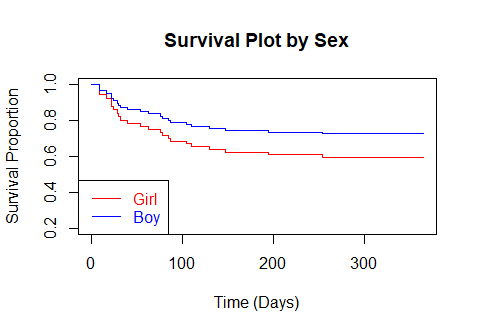
\includegraphics[scale=0.75]{C://Users//guild//Documents//Stats//PS04//Survival Plot.png}
\end{document}
